\documentclass[a4paper,12pt,french]{report}
\usepackage[utf8]{inputenc}
\usepackage[T1]{fontenc}
\usepackage{textcomp}
\usepackage{babel}
\usepackage{amsmath,amssymb}
\usepackage{minted}
\usepackage{array}
\usepackage{tabularx}
\usepackage{multirow}
% \usepackage{minipage}
%\usepackage[toc,pagee]{appendix}
\usepackage{graphicx}
\graphicspath{
	{images}
}
\usepackage{caption}
\usepackage[top=2cm,left=2cm,right=2cm,bottom=2cm,headsep=1.5cm]{geometry}
\usepackage[hidelinks]{hyperref}
\usepackage{xcolor}
\usepackage{bbold}
\usepackage{titlesec}
\usepackage{blindtext}
\usepackage{multicol}

\usepackage{fancyhdr} %en-tetes et bas de page
\pagestyle{fancy}
%\fancyhf{} % Efface les en-têtes et pieds de page par défaut

\usepackage[style=numeric,backend=bibtex, sorting=none]{biblatex}
%\addbibresource{TPMN.bib}

\usepackage{csquotes}

%Outils Mathématiques
\addto\captionsfrench{
    \renewcommand*{\chaptername}{Partie}
}
\newcommand{\N}{\mathbb{N}}
\newcommand{\R}{\mathbb{R}}
\renewcommand{\P}{\mathcal{P}}
\newcommand{\lsum}[2]{\sum\limits_{#1}^{#2}}
\newcommand{\x}{\times}
\renewcommand{\phi}{\varphi}
\renewcommand{\epsilon}{\varepsilon}

\newcommand{\norminf}[1]{\left\lVert {#1} \right\rVert _\infty}
\newcommand{\norm}[1]{\left\lvert {#1} \right\rvert}
\newcommand{\norme}[2]{\left\lVert {#1} \right\rVert_{#2}}


\DeclareMathOperator{\e}{\mathrm e}
\newcommand{\abs}[1]{\lvert#1\rvert}

\newtheorem{theorem}{Théorème}
\newtheorem{propo}{Proposition}
\newtheorem{prop}{Propriété}

% \renewcommand{\bf}{\textbf}

% ON MET DES ACCENTS SUR LES MAJUSCULES
% accent aigu : \' (apostrophe)
% accent grave : \` (accent grave en-dessous de £)
% accent circonflexe : \^
% tréma : \"

%PAGE DE GARDE
\author{Rozenn \textsc{Le Bihan}
\\Axel \textsc{Raynond}
\\Rémy \textsc{Labarre}
\\Matys \textsc{Bieche}
\\Alexandre \textsc{Amaro Monteiro}\vskip0.1cm
Txomin \textsc{bisbau}}
\date{2023-2024}
\title{{Exercices sur les problèmes aux limites}}

% En-tête personnalisé
\fancypagestyle{plain}{
    \fancyhead[L]{
\includegraphics[height=0.7cm]{figures/logosea.png}}
    \fancyhead[R]{
\includegraphics[height=1cm]{figures/logodassault.png}}
    \fancyhead[C]{Dassault UAV Challenge} %en-tête au milieu
}
\lhead{
\includegraphics[height=0.7cm]{figures/logosea.png}} % En-tête à gauche
\rhead{
\includegraphics[height=1cm]{figures/logodassault.png}} % En-tête à droite
\chead{Dassault UAV Challenge}
\renewcommand{\headrulewidth}{1pt} % Épaisseur de la barre horizontale

\begin{document}

\begin{titlepage}
    \makeatletter
    \noindent
    
\includegraphics[height=1cm]{figures/logosea.png}
    
\includegraphics[height=1cm]{figures/logouniv.png}
    \hfill
    
\includegraphics[height=1.6cm]{figures/logodassault.png}
    \vfill
    \begin{center}
        \rule{0.95\textwidth}{2pt}\vspace{0.3\baselineskip}\\
        \LARGE \textbf{\textsc{- Dassault UAV Challenge -}\vspace{0.51\baselineskip}\\ \'Equipe Sea'gogne} \normalsize\\
        \rule{0.95\textwidth}{2pt}\vskip1cm
        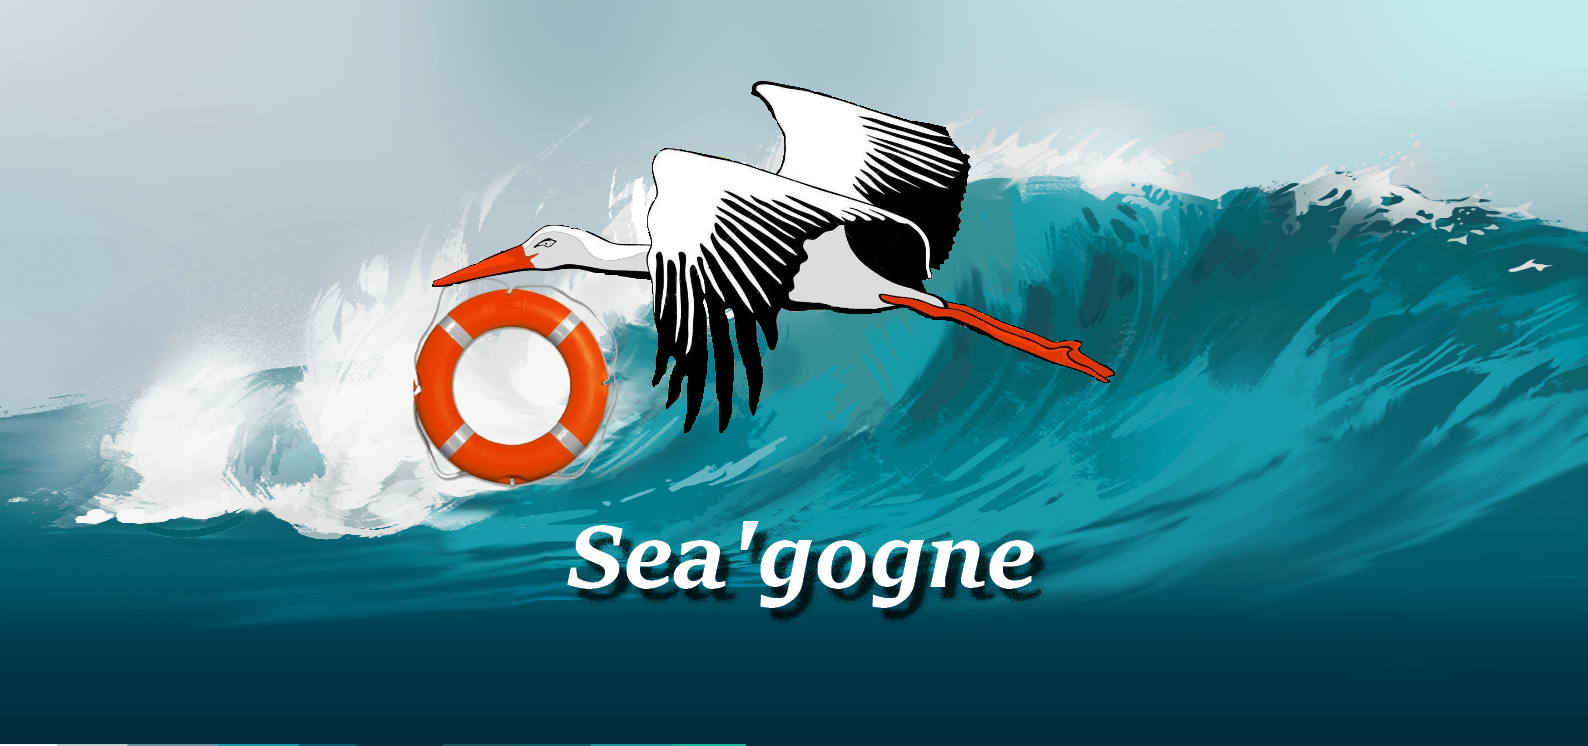
\includegraphics[height=7cm]{figures/seagogne.png}\vskip1cm
        {\large\@author}\vskip2cm
    \end{center}
    \textbf{Professeur référent :}
    \\Monsieur \textsc{Ostre}, Maître de conférence à SeaTech
    \vskip0.5cm
    \centering
    \@date
    \makeatother
\end{titlepage}

\thispagestyle{empty}

\pagenumbering{roman}

\chapter*{Remerciements}

Nous remercions tout d'abord notre professeur référent M.\textsc{Ostre} pour son enthousiasme et son aide tout long de notre projet.\newline

Nous souhaitons également remercier notre école d'ingénieur SeaTech pour les locaux et le matériel à disposition.\newline

Nous remercions tout particulièrement l'équipe encadrante du \textsc{Dassault} UAV Challenge pour l'opportunité qu'ils nous donnent en participant à cette compétition et les dispositifs mis en place pour nous.

%Sommaire
\tableofcontents

\pagenumbering{arabic}

\begin{abstract}
    Dans le cadre de la compétition \textsc{Dassault} UAV Challenge, notre équipe s'attelle à la conception d'un drone VTOL dédié aux opérations de sauvetage en mer. De la sélection de la structure au dimensionnement précis des composants, chaque étape de notre processus de développement est réalisée de manière à créer un drone aussi performant que possible, tout en répondant aux exigences rigoureuses définies par la compétition.

    Grâce à la diversité de nos compétences et à nos recherches approfondies, nous avons fusionné nos connaissances dans le cadre de ce projet pluridisciplinaire. De la modélisation à la simulation, en passant par la programmation, l'automatisation et l'électronique, chaque domaine a été abordé avec une attention particulière. Notre objectif est de présenter un drone qui allie l'expertise technique à une approche globale pour répondre efficacement aux défis complexes du sauvetage en mer. \vskip4cm

    \begin{center}
        \bfseries Abstract
    \end{center}

    \noindent
    \textcolor{red}{traduire}
\end{abstract}

\chapter*{Introduction}
\addcontentsline{toc}{chapter}{\protect\numberline{}Introduction}

Dans le cadre de la compétition organisée par Dassault, nous sommes fiers de présenter notre drone conçu pour répondre à des besoins en sauvetage en mer. Inspiré par l'engagement envers l'innovation et la sécurité, notre équipe a développé un drone à décollage vertical et atterrissage (VTOL) qui redéfinit les normes en matière de missions de sauvetage en milieu maritime.\newline

Face aux défis complexes posés par les situations d'urgence en mer, notre drone VTOL offre une solution polyvalente et efficace. Doté de capacités de décollage vertical, ce drone peut être rapidement déployé depuis diverses plateformes. Sa conception a été minutieusement élaborée pour garantir une performance optimale tout en maintenant une empreinte écologique minimale.\newline

Au-delà de la technologie de pointe, notre drone de sauvetage en mer est équipé de capteurs, d’une caméra et de systèmes de communication. Ces fonctionnalités avancées permettent au drone de localiser rapidement et avec précision les personnes en détresse en mer, fournissant ainsi des informations cruciales pour coordonner des opérations de sauvetage rapides et efficaces.\newline

Nous sommes impatients de démontrer comment notre drone VTOL peut répondre aux exigences et à sa mission de sauvetage en mer. Notre engagement envers l'innovation, la sécurité et l'efficacité se reflète dans chaque aspect de ce projet.

\chapter{Présentation}

\section{Contexte et mission : sauvetage en mer}

Tout d'abord, notre école d'ingénieur SeaTech étant situé à Toulon, première base navale française et premier port de défense d'Europe, et ayant une identité tournée vers le maritime, il nous a paru naturel d'orienter la mission de notre drone vers ce dernier. De plus, sur la côte d'Azur, nous imaginons que les besoins de sauvetage en saison estivale sont amplifiés. C'est pourquoi, nous voulons que notre drone puisse apporter assistance à une personne en mer. Cela passe par sa détection, avec le renvoi d'une coordonnée GPS aux sauveteurs, et par l'assistance d'une bouée de sauvetage en attendant les sauveteurs. Ces informations sont représentées sous un diagramme bête à corne ci-dessous (\ref{bete}).
\bigskip

\begin{figure}[h]
    \centering
    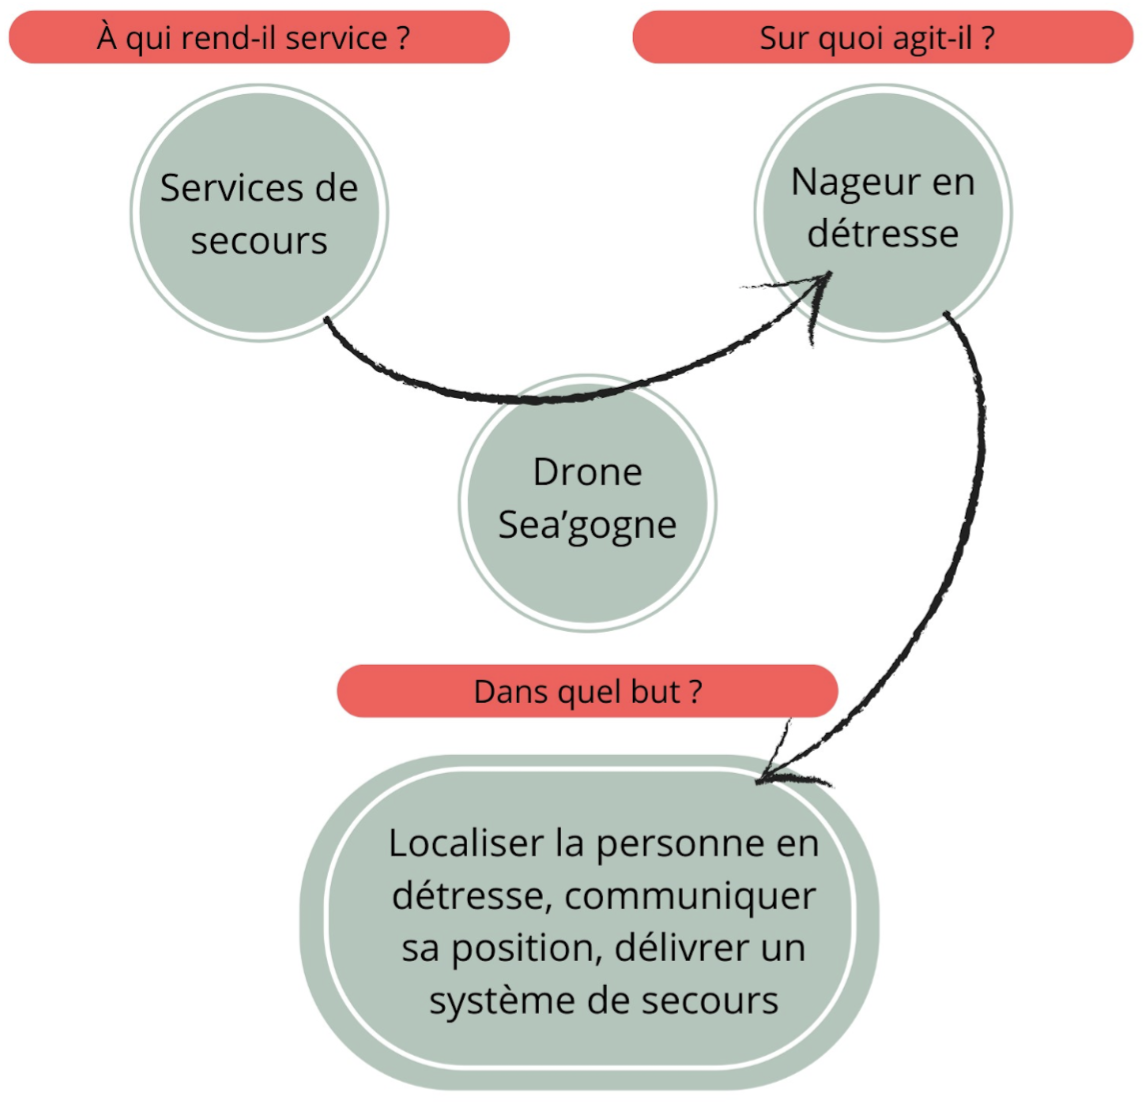
\includegraphics[height=10cm]{figures/bete.png}
    \caption{Diagramme bête à corne}
    \label{bete}
\end{figure}

\section{Fonctionnalités et diagrammes techniques}

\subsubsection*{Diagramme des interacteurs}

La réalisation de notre drone nécessite de comprendre les liens qui l’unissent aux différents acteurs qu’il rencontrera, dans le but de déterminer l’environnement dans lequel il devra évoluer. Cet environnement conditionne les fonctions de notre drone, divisées en deux types : les principales (FP) et contraintes (FC).

\begin{figure}[h]
    \centering
    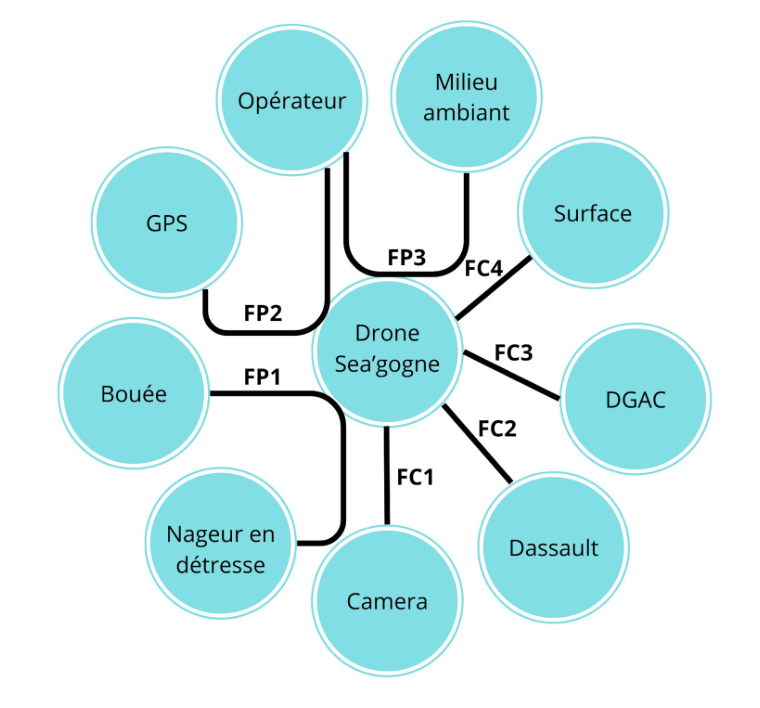
\includegraphics[height=10cm]{figures/diagex.png}
    \caption{Diagramme des interacteurs}
    \label{diagex}
\end{figure}

\begin{table}[H]
    \centering
    \begin{tabularx}{14cm}{|c|p{12.25cm}|}
        \hline
        \textbf{FP1} & \textbf{Piloter le drone dans son environnement}                                                                                  \\
        \hline
        \textbf{FP2} & \textbf{Larguer la bouée de manière sûre et précise au nageur}                                                                    \\
        \hline
        \textbf{FP3} & \textbf{Fournir la position du drone à l’opérateur et permettre à l’appareil de se rendre à un point précis}                      \\
        \hline
        \textbf{FC1} & \textbf{Visualiser l’environnement et détecter le nageur en détresse afin de se positionner}                                      \\
        \hline
        \textbf{FC2} & \textbf{Respecter les contraintes obligatoires et importantes imposées par Dassault dans le cadre du Dassault UAV Challenge 2024} \\
        \hline
        \textbf{FC3} & \textbf{Respecter les normes de la DGAC appliquées aux UAV de catégorie C2}                                                       \\
        \hline
        \textbf{FC4} & \textbf{Décoller sur une distance courte et tout type de sol}                                                                     \\
        \hline
    \end{tabularx}
    \caption{Tableau des fonctions : principales et complémentaires}
\end{table}

\newpage
\subsubsection*{Contraintes détaillées}

Les exigences que nous détaillons ci-dessous correspondent aux valeurs du prototype et peuvent donc être imparfaites ou simplifiées. Certaines valeurs seront donc sûrement à modifier à la suite de nos tests.
\bigskip

\begin{table}[H]
    \begin{tabularx}{18.5cm}{|p{2cm}|l|p{4.5cm}|p{2cm}|X|}
        \hline
        \textbf{Fonctions de service} & \textbf{Critères d’appréciations}    & \textbf{Niveaux d’appréciations} & \textbf{Limite d’acceptation} & \textbf{Classe} \\
        \hline
        \multirow{5}{*}{\textbf{FP1}}
                                      & Propulsion (puissance moteur)        & 2x 300W                          & >2 x 300W                     & F1              \\
                                      & Vitesse horizontal                   & 80 km/h                          &                               & F2              \\
                                      & Vitesse vertical                     & 2m/s                             &                               & F2              \\
                                      & Altitude (niveau mer)
                                      & 120m                                 & min 80 m                         & F1                                              \\
                                      & Portée communication                 & > 500m                           &                               & F1              \\
        \hline
        \multirow{3}{*}{\textbf{FP2}}
                                      & Capacité de charge                   & 500g                             &                               & F1              \\
                                      & Dispositif de largage                & Gachette + Filin                 &                               & F1              \\
                                      & Précision largage                    & +/-30cm                          &                               & F1              \\
        \hline
        \textbf{FP3}                  & Récepteur GPS                        & Position exacte                  & ± 2m                          & F1              \\
        \hline
        \multirow{2}{*}{\textbf{FC1}}
                                      & Caméra                               & Résolution de 1920x1080          &                               & F1              \\
                                      & Précision du positionnement          & Position exacte                  & ± 0.5m                        & F1              \\
        \hline
        \multirow{7}{*}{\textbf{FC2}}
                                      & Bouton d'arrêt d’urgence             & instantané                       &                               & F0              \\
                                      & Suivre une trajectoire               & Précision de 3m                  &                               & F0              \\
                                      & Respecter un périmètre de vol        & 100x50x120m                      &                               & F0              \\
                                      & Capacité de vol autonome
                                      &                                      &                                  & F0                                              \\
                                      & Retour du drone si perte de signal   &                                  &                               & F0              \\
                                      & Retour niveau batterie               & Précision au pourcentage         &                               & F1              \\
                                      & Retour paramètres de vol             &                                  &                               & F1              \\
        \hline
        \multirow{3}{*}{\textbf{FC3}}
                                      & Poids                                & < 4kg (classe C2)                &                               & F0              \\
                                      & Dispositif de signalement à distance & Portée de 1km                    &                               & F0              \\
                                      & Fonction de géovigilance             &                                  &                               & F0              \\
        \hline
        \multirow{2}{*}{\textbf{FC4}}
                                      & Système VTOL                         &                                  &                               & F0              \\
                                      & Switch mode avion-hélicoptère        & Durée : 2 secondes               &                               & F1              \\
        \hline
    \end{tabularx}
    \caption{Tableau des contraintes détaillées}
\end{table}

\newpage
\subsubsection*{Diagramme FAST}

\begin{figure}[h]
    \centering
    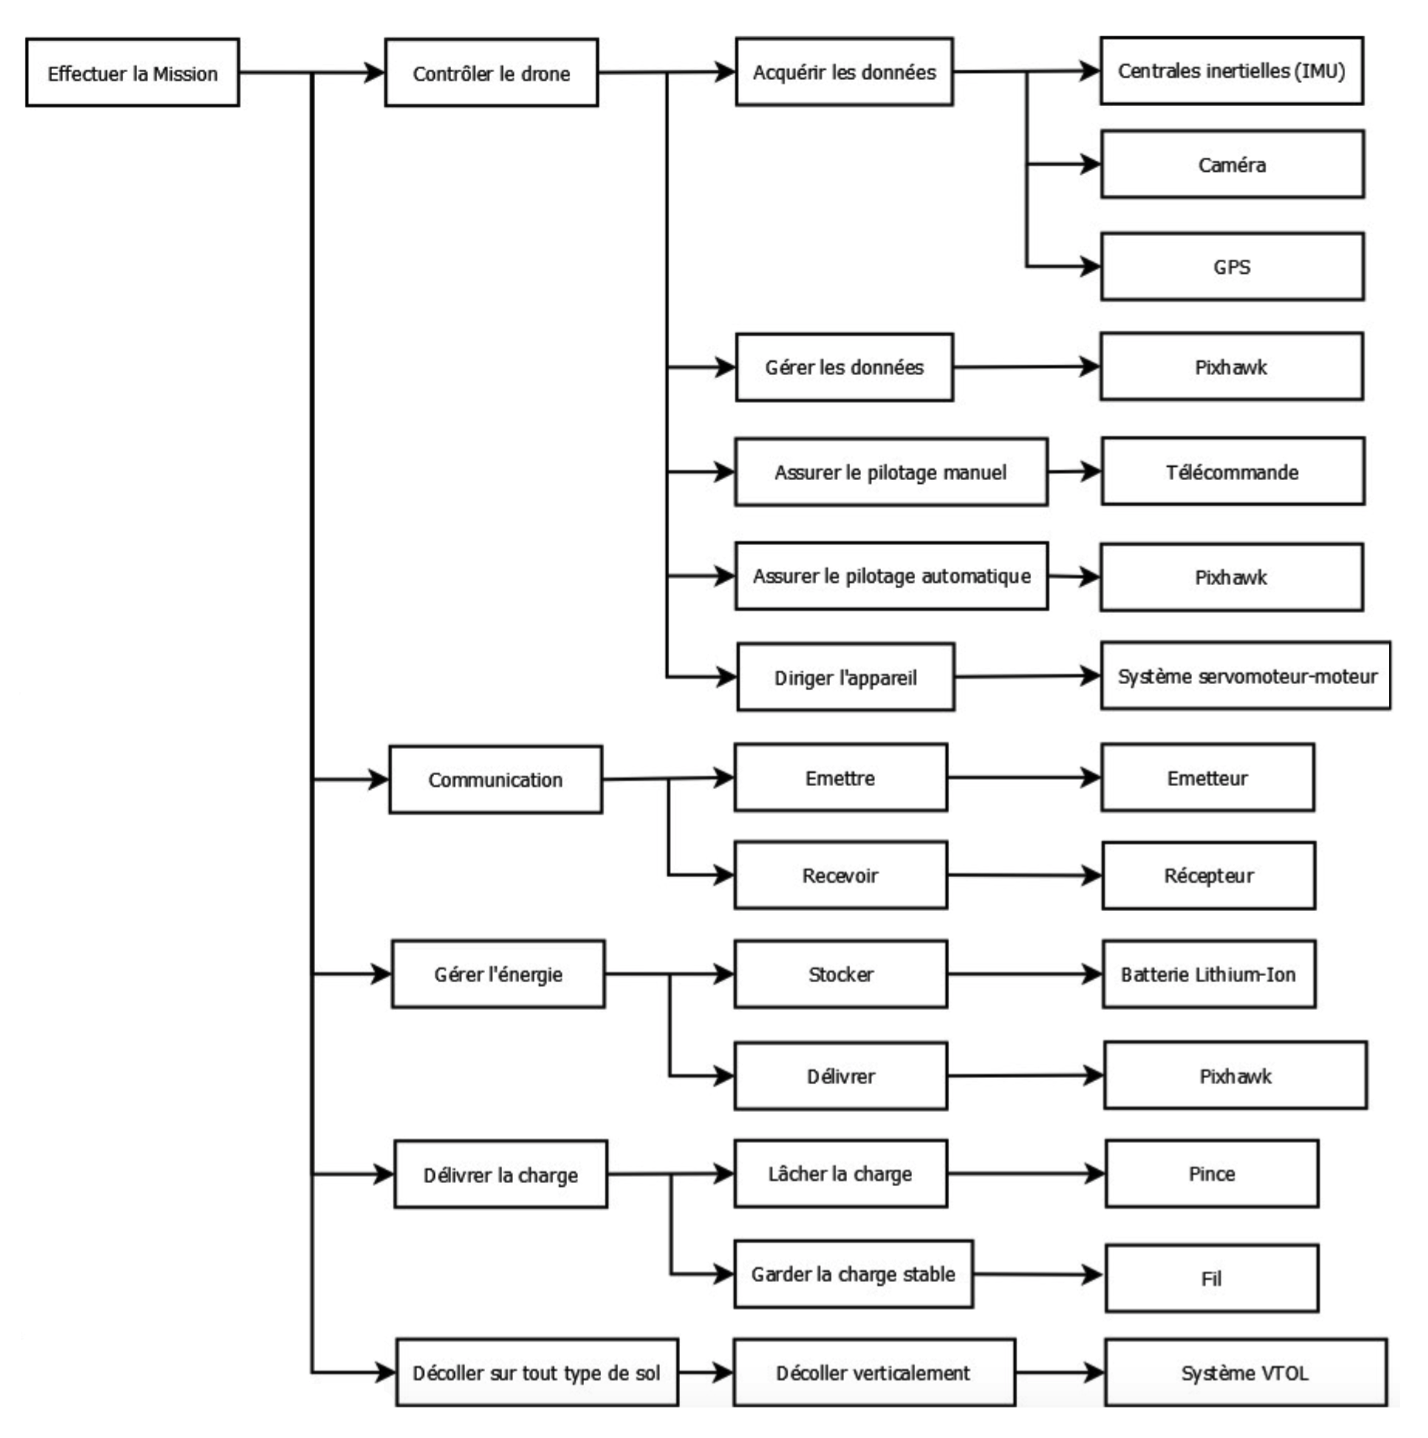
\includegraphics[height=16cm]{figures/fast.png}
    \caption{Diagramme FAST}
    \label{fonctions}
\end{figure}

\newpage
\subsubsection{Diagramme cinématique}
Nous avons réalisé le diagramme cinématique de notre drone afin de visualiser les différents acteurs.
\begin{figure}[h]
    \centering
    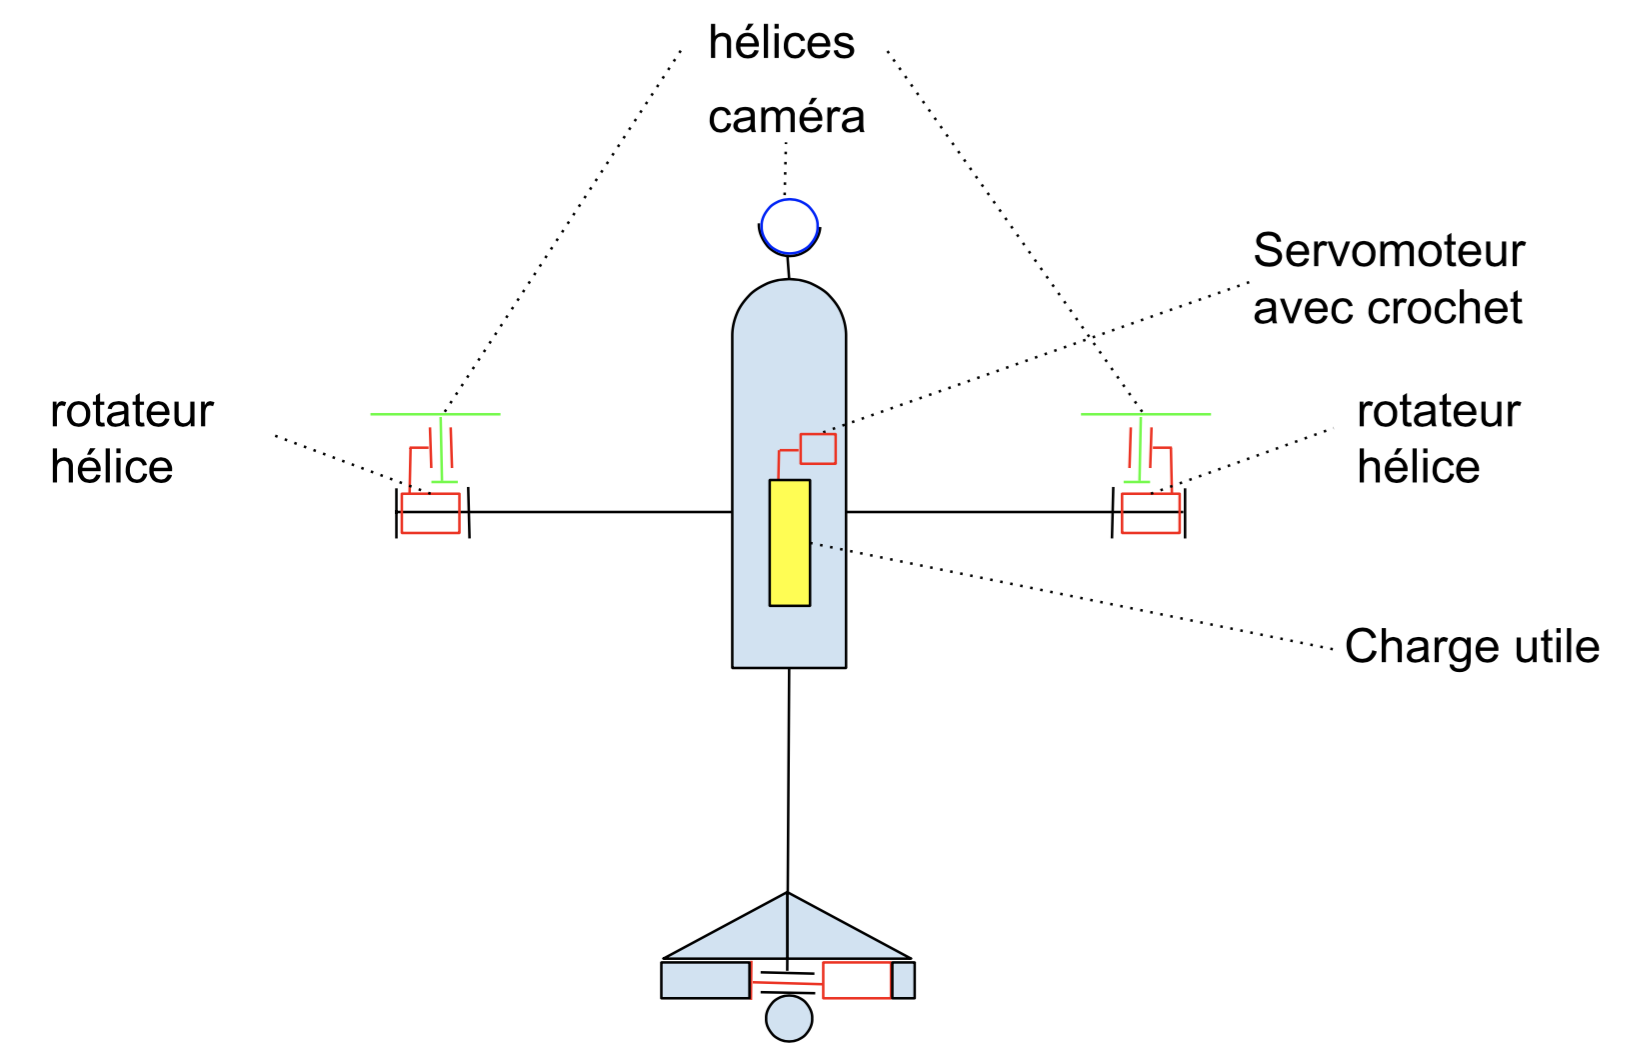
\includegraphics[height=10cm]{figures/cine.png}
    \caption{Diagramme cinématique}
    \label{cine}
\end{figure}

Nous avons fait le choix de ne pas avoir de parties mobiles sur la voilure, laissant ainsi les servomoteurs et les moteurs aux extrémités des ailes gérer les axes de roulis, tangage et lacet. De la même manière, l’empennage vertical et horizontal est fixe. Le système de largage est quant à lui composé d’un servomoteur et est détaillé dans la partie (\ref{larg}). La caméra est située à l’avant de l’appareil et ne sera pas mobile, elle est orientée à la verticale de l’appareil pour pouvoir être placé au-dessus de la victime.

\chapter{Réalisation fonctionnelle du drone}

\section{Structure du drone}

Dans cette partie, nous présenterons la structure du drone et les choix qui ont été fait quant à cette dernière.

\subsection{Fuselage}

Pour le fuselage de l’avion, nous avons pensé à une base simple et modifiable selon l’avancée du projet. Elle reprend l’idée générale de la calandre du VTOL développée par le Youtuber Tom Stanton. Pour allier tous nos objectifs de mission, le fuselage  comprend plusieurs éléments qui pourront évoluer au fil de notre conception. La structure a été adaptée pour fixer une plateforme Pixhawk à l’horizontale, mais contiendra aussi la batterie et l’électronique embarqué. Elle comprend :

\begin{itemize}
    \item Une clé d’aile comprenant une fixation pour le tube avec une inclinaison de 3 degrés ainsi qu’un espace central pour  passer les fils des moteurs à l'électronique. L'inclinaison de 3 degrés de la clé d'aile va permettre d’optimiser la portance de l’aile sans en exagérer la traînée. De plus, elle a été étudiée pour résister aux contraintes mécaniques appliquées par les tubes sur la structure.
          \begin{figure}[h]
              \centering
              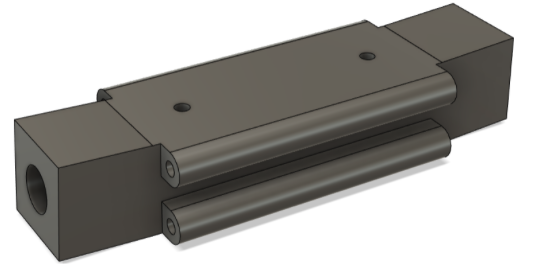
\includegraphics[height=5cm]{figures/cle.png}
              \caption{Clé d'aile}
          \end{figure}
    \item 2 plaques extérieures qui vont représenter une première protection pour l’électronique embarqué.
    \item Une pièce de fixation de queue permettant la fixation de l’ensemble tube-empennage. Elle a été conçue pour allier une réduction maximale de sa masse et une résistance maximale.
          \begin{figure}[h]
              \centering
              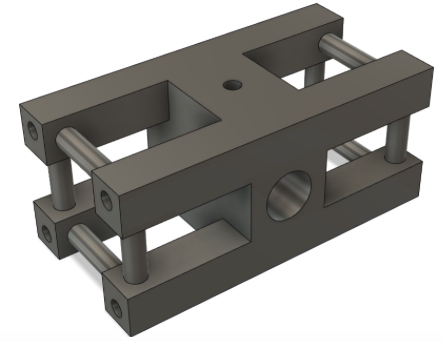
\includegraphics[height=5cm]{figures/arr.png}
              \caption{Clé d'aile}
          \end{figure}
          \newpage
    \item Un fond avec une fixation des composants électroniques et de la batterie.
\end{itemize}

Avec notamment la partie inférieure qui pourra évoluer pour avoir un emplacement pour la caméra et une adaptation pour le système de largage qui sera developpé dans la partie (\ref{larg}).\newline

L'impression 3D de la structure offre une fabrication personnalisée, rapide et économique. Elle va nous permettre la réalisation de pièces essentielles avec de la résine thermoplastique.

Nous avons choisi ce mode de réalisation car il favorise les essais avec une réalisation rapide. Cela nous permet aussi d’avoir des pièces plus légères tout en réduisant les déchets de production.\newline

En somme, le calandre du VTOL est une composante essentielle qui répond à la fois à des contraintes fonctionnelles, de sécurité et d'esthétisme. Elle assure à la fois une structure rigide et la protection des systèmes embarqués tout en contribuant à l'aérodynamisme du drone.


\subsection{Aile}

\subsubsection*{Profil et dimensionnement des ailes}

Pour le profil de nos deux ailes, nous avons choisi le profil NACA 4412. En effet, c'est un profil qui est stable sans décrochage brutal du coefficient de portance (\ref{cz}). D'autre part, dans notre cas d'utilisation, nous ne faisons pas de voltige donc il n'aurait pas été judicieux de prendre un profil symétrique par exemple.\newline

\begin{figure}[h]
    \centering
    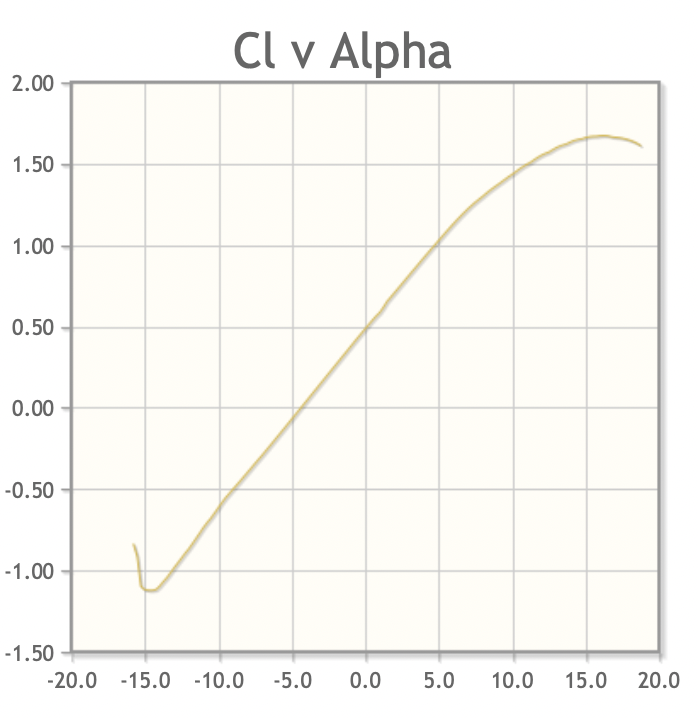
\includegraphics[height=8cm]{figures/cz.png}
    \caption{Courbe du coefficient de portance en fonction de l'incidence}
    \label{cz}
\end{figure}

Nous avons par la suite calculé la surface à l'air de notre aile. Pour cela, nous avons utilisé l'expression de la portance.

$$ F_p=\frac{1}{2}\rho S C_z v^2$$

Avec $C_z$ le coefficient de portance.

Nous déterminons ainsi la surface.
$$S=\frac{2F_p}{\rho C_z v^2}$$

Nous réalisons les calculs lorsque la force de portance égalise celle du poids du drone : $F_p=P.$ Avec une masse de $m=1$kg, nous trouvons $F_p=9,81$N. Nous choisissons un angle d'incidence de $6°$ ce qui nous donne un coefficient de portance $C_z=1,2$.\newline

Nous trouvons après application numérique une surface de $S=1,265$$m^2$, avec $\rho=1,292$kg/$m^3$ et $v=10$m/s.\newline

    Nous décidons ainsi de dimensionner notre aile de $60cm$ de longeur et $20cm$ de large.

\subsubsection*{Conception de l'aile}

Notre aile est conçu en polystyrène. Elle est découpée à l'aide d'une découpeuse à fil chaud. Après avoir réalisé la modélisation sur Catia du profil de l'aile, nous l'envoyons à la découpeuse.

\begin{figure}[h]
    \centering
    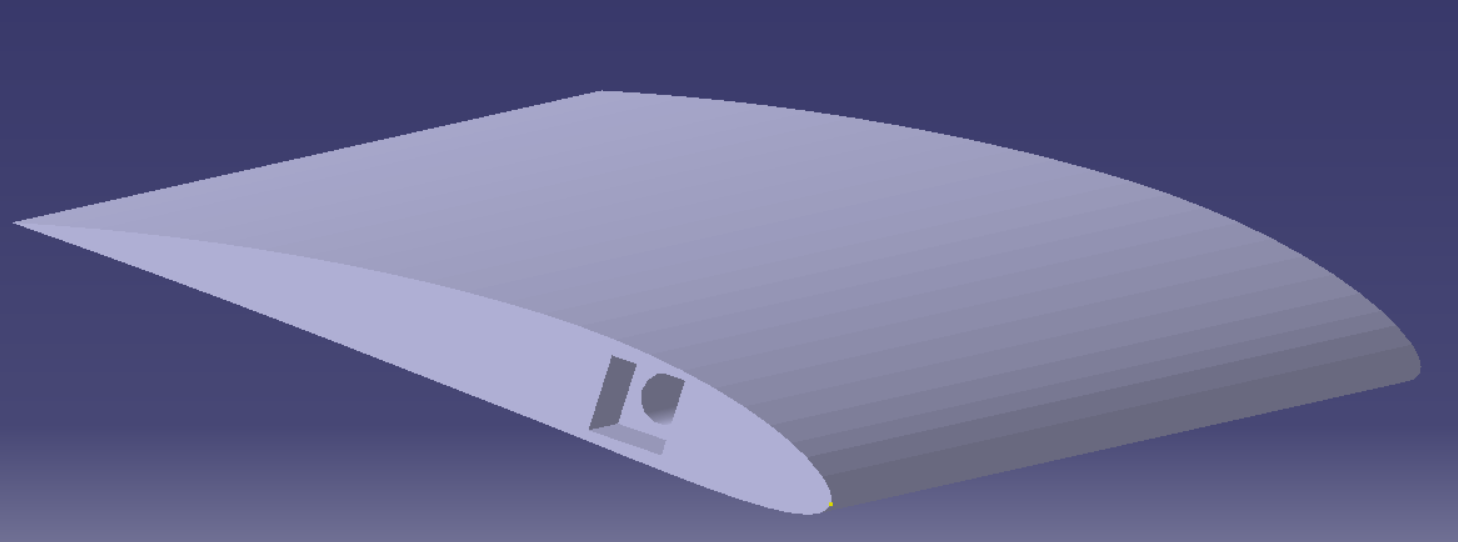
\includegraphics[height=5cm]{figures/ailec.png}
    \caption{Modélisation de l'aile sur CatiaV5}
\end{figure}

\textcolor{red}{photo Catia, photo résultat}

\subsection{Systèmes moteur}

Le système moteur a deux objectifs : diriger l'appareil en vol horizontal tout en assurant sa stabilité, et assurer la translation vertical du drone en mode hélicoptère. Nous nous sommes alors penchés sur la manière de concevoir le socle du moteur sur l’aile permettant d'assurer ces tâches. Sachant qu’à notre disposition nous possédons un moteur (Insérer référence), l’architecture du socle moteur a été construite sur cette base. Le système moteur ainsi conçu doit répondre aux critères de notre mission, soit lui permettre de faire décoller l’appareil à la verticale puis de changer sa position de vol pour passer à un vol horizontal. \newline

L’idée consiste à permettre la rotation du socle moteur sur le support de l’aile, tout en minimisant l’espace qu’il utilise et en l’empêchant de glisser longitudinalement sur le support de l’aile. La rotation s’effectue à l’aide de deux engrenages. Le train d’entrée est mis en rotation à l’aide d’un servomoteur (référence petit moteur). Il faut donc un support pour celui-ci.\newline

De là, 3 pièces sont à créer :
\begin{itemize}
    \item Le support moteur (pièces 1)
    \item Support servomoteur (pièce 2)
    \item Des cales (pièces 3)
    \item Un engrenage (pièce 4)
\end{itemize}

Les pièces sont ainsi réalisées sous CatiaV5.

\begin{figure}[h]
    \centering
    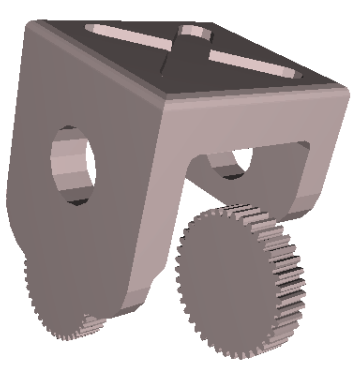
\includegraphics[height=5cm]{figures/mot1.png}
    \caption{Modélisation des pièces 1 et 4}
\end{figure}

\begin{figure}[h]
    \centering
    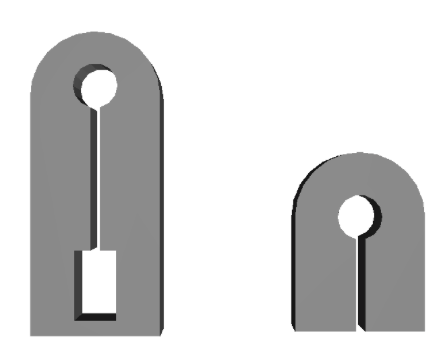
\includegraphics[height=5cm]{figures/mot2.png}
    \caption{Modélisation des pièces 2 et 3}
\end{figure}

\subsection{Structure entre le fuselage et les moteurs : tubes}

Nos sytèmes moteur sont reliés au fuselage par l'intermédiaire de tubes creux en aluminium. Pour cela, nous devons mener une étude pour choisir judicieusement les dimensions de ce tube.\newline

Tout d'abord, étant donné que notre aile fait une longueur de 60cm, nous choisissons de prendre un tube d'une longueur de 70cm. En effet, nous devons prendre en compte également le support en bout de tube en plus de l'aile.\newline

Dans un second temps, nous devons choisir le diamètre du tube. Nous avons donc fait une étude de résitance des matériaux afin de le déterminer en fonction de la limite d'élasticité de l'aluminium et les paramètres de notre système.\newline

Cela nous a amener à calculer le diamètre dans trois cas (\ref{flex}):
\begin{itemize}
    \item Cas 1 : drone à l'arrêt, le tube supporte la force du poids (P),
    \item Cas 2 : drone en vol vertical, le tube supporte la force du poids (P) et la force moteur (F),
    \item Cas 3 : drone en vol horizontale, le tube suporte la force du poids (P), la force moteur (F) et la force linéique de la portance (w) sur toute l'aile.
\end{itemize}

\begin{figure}[h]
    \centering
    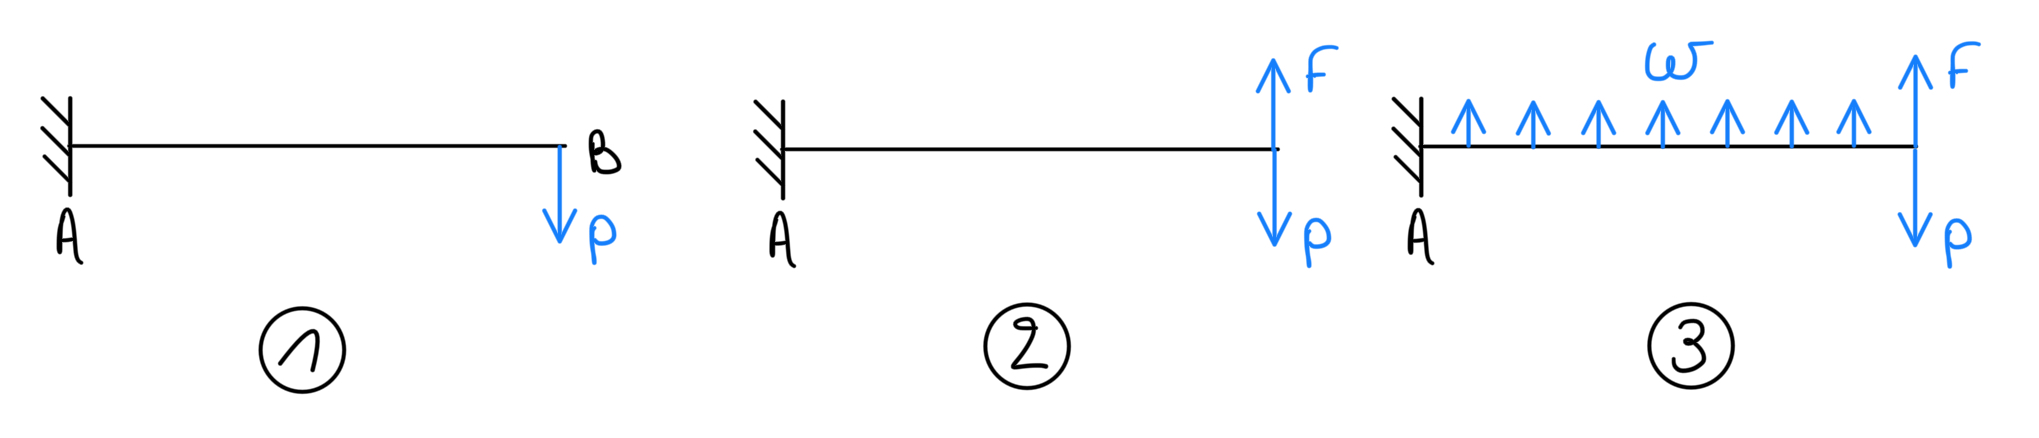
\includegraphics[height=3cm]{figures/flexion.jpeg}
    \caption{Schémas des 3 cas d'étude de poutre en flexion}
    \label{flex}
\end{figure}

\textcolor{red}{résultat}

Pour confirmer nos calculs théoriques, nous avons décidé de faire une simulation sur Abaqus.\newline

\textcolor{red}{résultat}

Nous avons également réalisé l'expérience afin de valider notre structure.\newline

\textcolor{red}{résultat}


\subsection{Empennage}

L'empennage de notre drone est un empennage classique position basse. Cette empennage permet de venir stabiliser le vol de notre drone. L'empennage, comme les ailes, est en polystyrène. Il est découpé au fil chaud.

\begin{figure}[h]
    \centering
    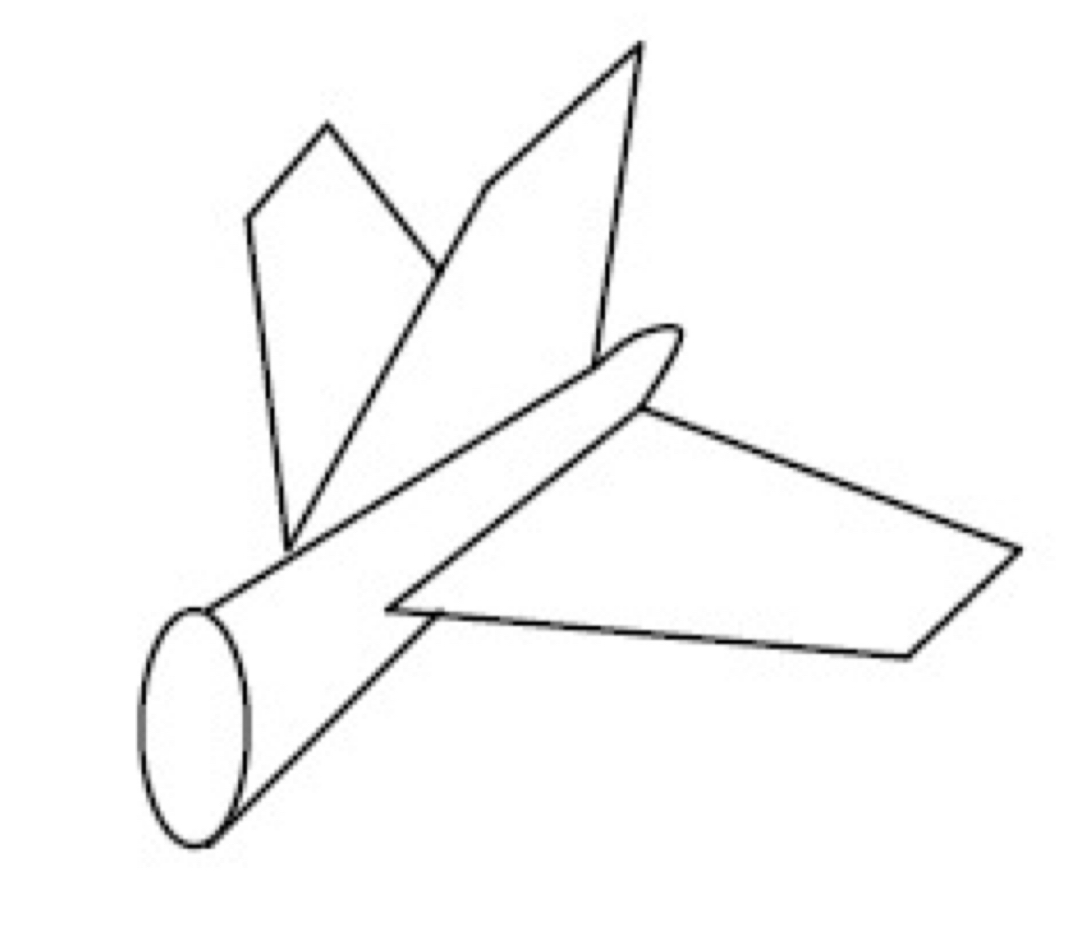
\includegraphics[height=4cm]{figures/emp.jpeg}
    \caption{Représentation de l''empennage}
    \label{flex}
\end{figure}

\newpage
\section{Contrôle du drone}

\subsection{Système électronique}

\subsection{Interface de commande}

\subsection{Automatisation}

\chapter{Réalisation de la mission : systèmes de sauvetage}

\section{Système de détection}

Notre mission consiste à envoyer le drone de manière autonome pour déposer une bouée à une personne en mer. Nous devons avoir un moyen de détecter les humains dans un périmètre donné. Nous avons donc opté pour une détection par caméra de la personne. Le choix le plus simple et le mieux adapté serait d'utiliser une caméra thermique pour détecter les zones chaudes. Il suffit donc de repérer ces zones et d'envoyer une image de confirmation à la station de contrôle pour s'assurer qu'il s'agit bien de la personne à secourir. Cela présente l'avantage d'être très simple à mettre en place et fonctionne de jour comme de nuit. Cependant, le coût de ces caméras est exorbitant, donc il nous est impossible d'en acquérir une d'une résolution suffisante cette année.\newline

Nous avons donc opté pour une approche avec une caméra classique couplée à un algorithme d'apprentissage supervisé de détection d'objet. Afin de déterminer si la technique pouvait fonctionner, nous avons pris nos nageurs les moins frileux et les avons photographiés dans la mer sous différents angles. Au total, nous avons recueilli plus de 1000 images que nous avons annotées avec une seule classe (noyé), soit un total de 2000 instances de nageurs que nous avons fournies à notre intelligence artificielle. Nous avons utilisé YOLOv8, car c'est la version la plus récente de la série YOLO et qu'elle est plus simple à entraîner que ses prédécesseurs tels que Darknet YOLO.
\bigskip
\begin{figure}[h]
    \begin{minipage}{0.5\textwidth}
        \centering
        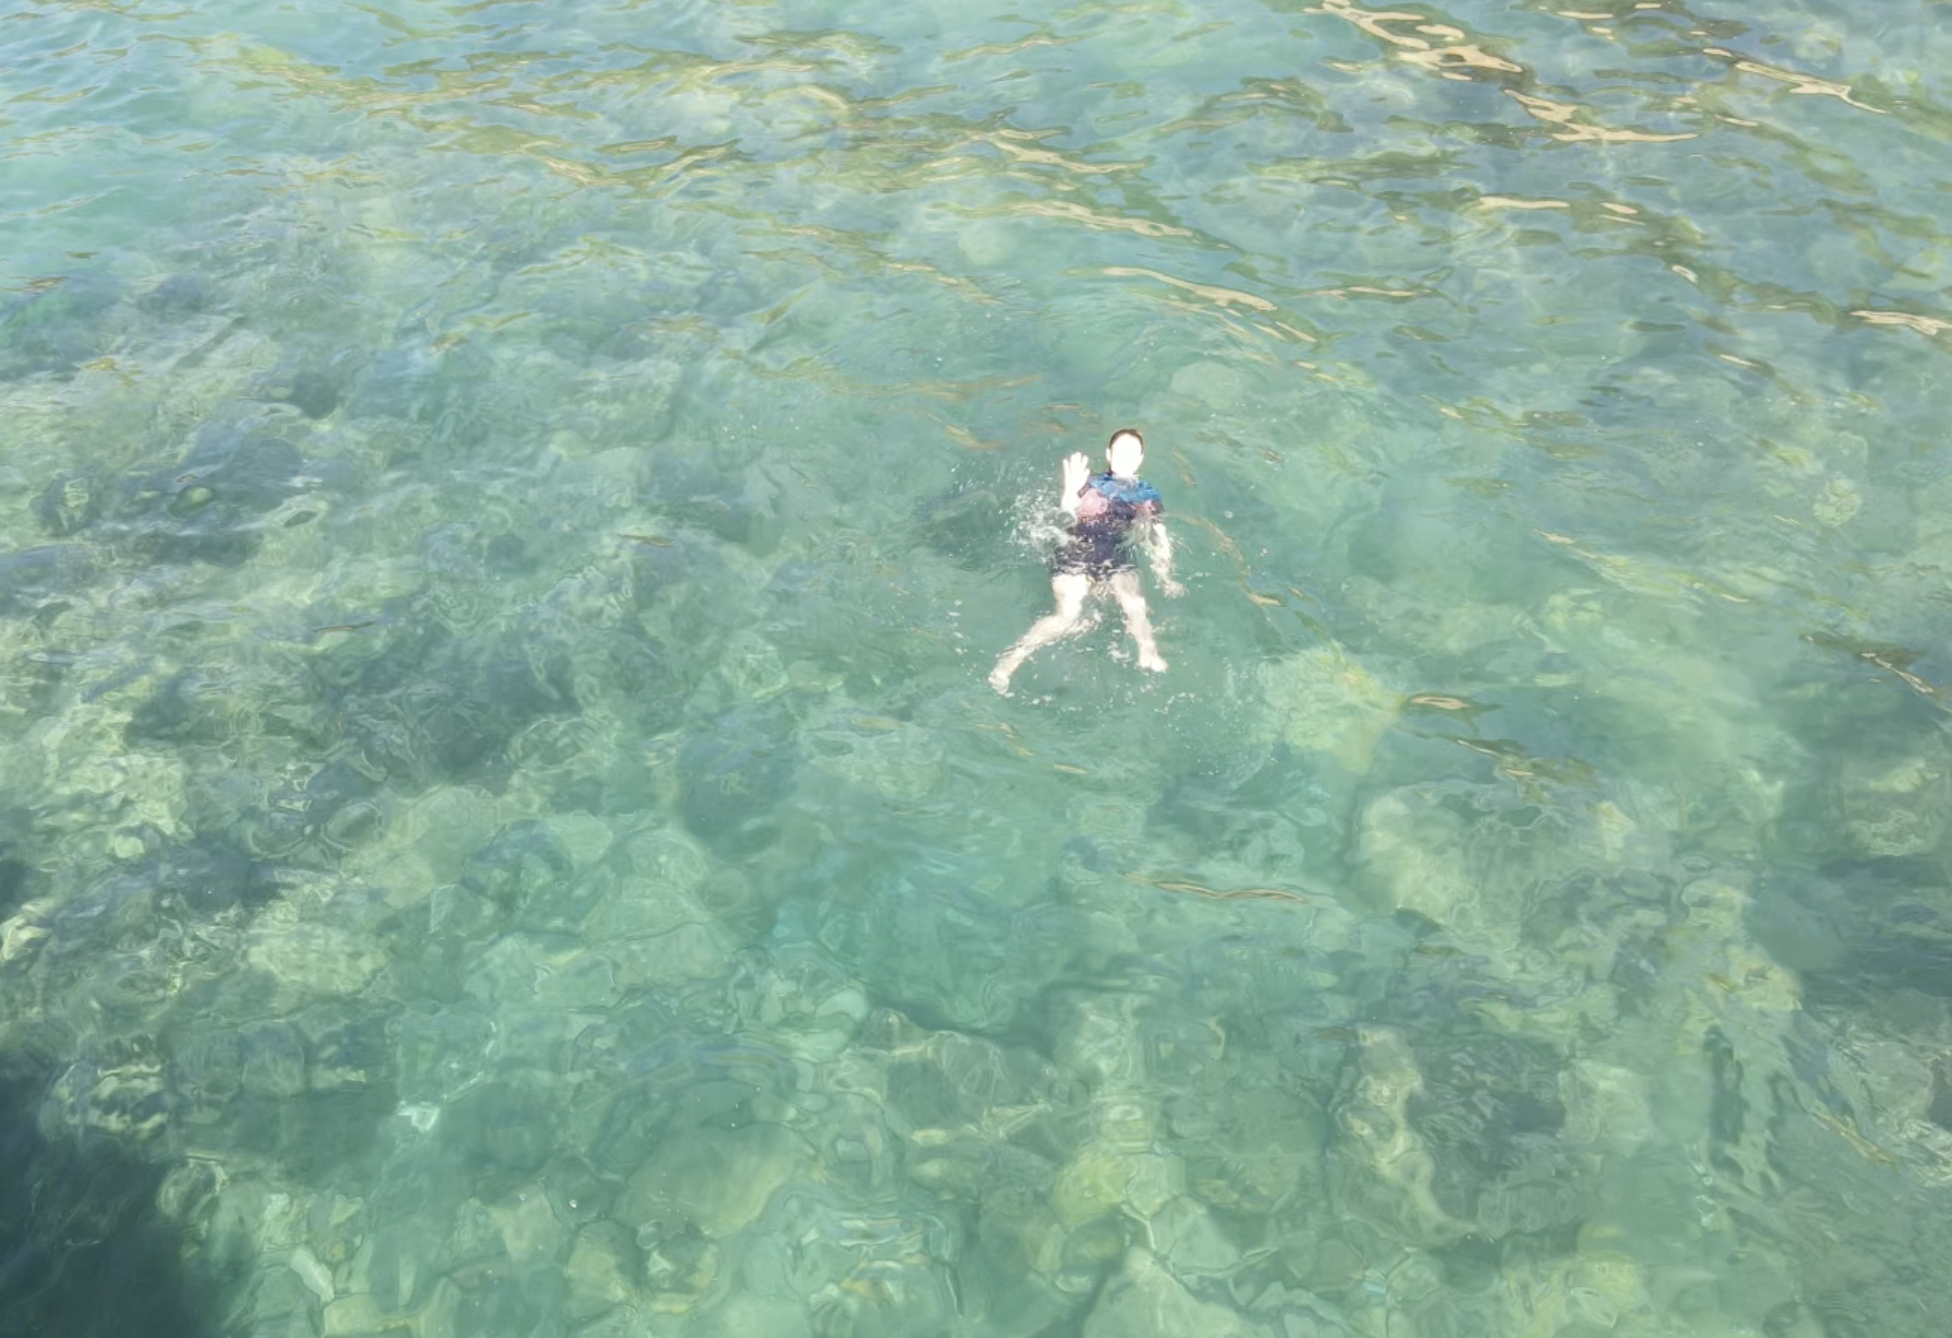
\includegraphics[height=4cm]{figures/vid.png}
        \caption{Image d'origine}
        \label{image}
    \end{minipage}%
    \begin{minipage}{0.5\textwidth}
        \centering
        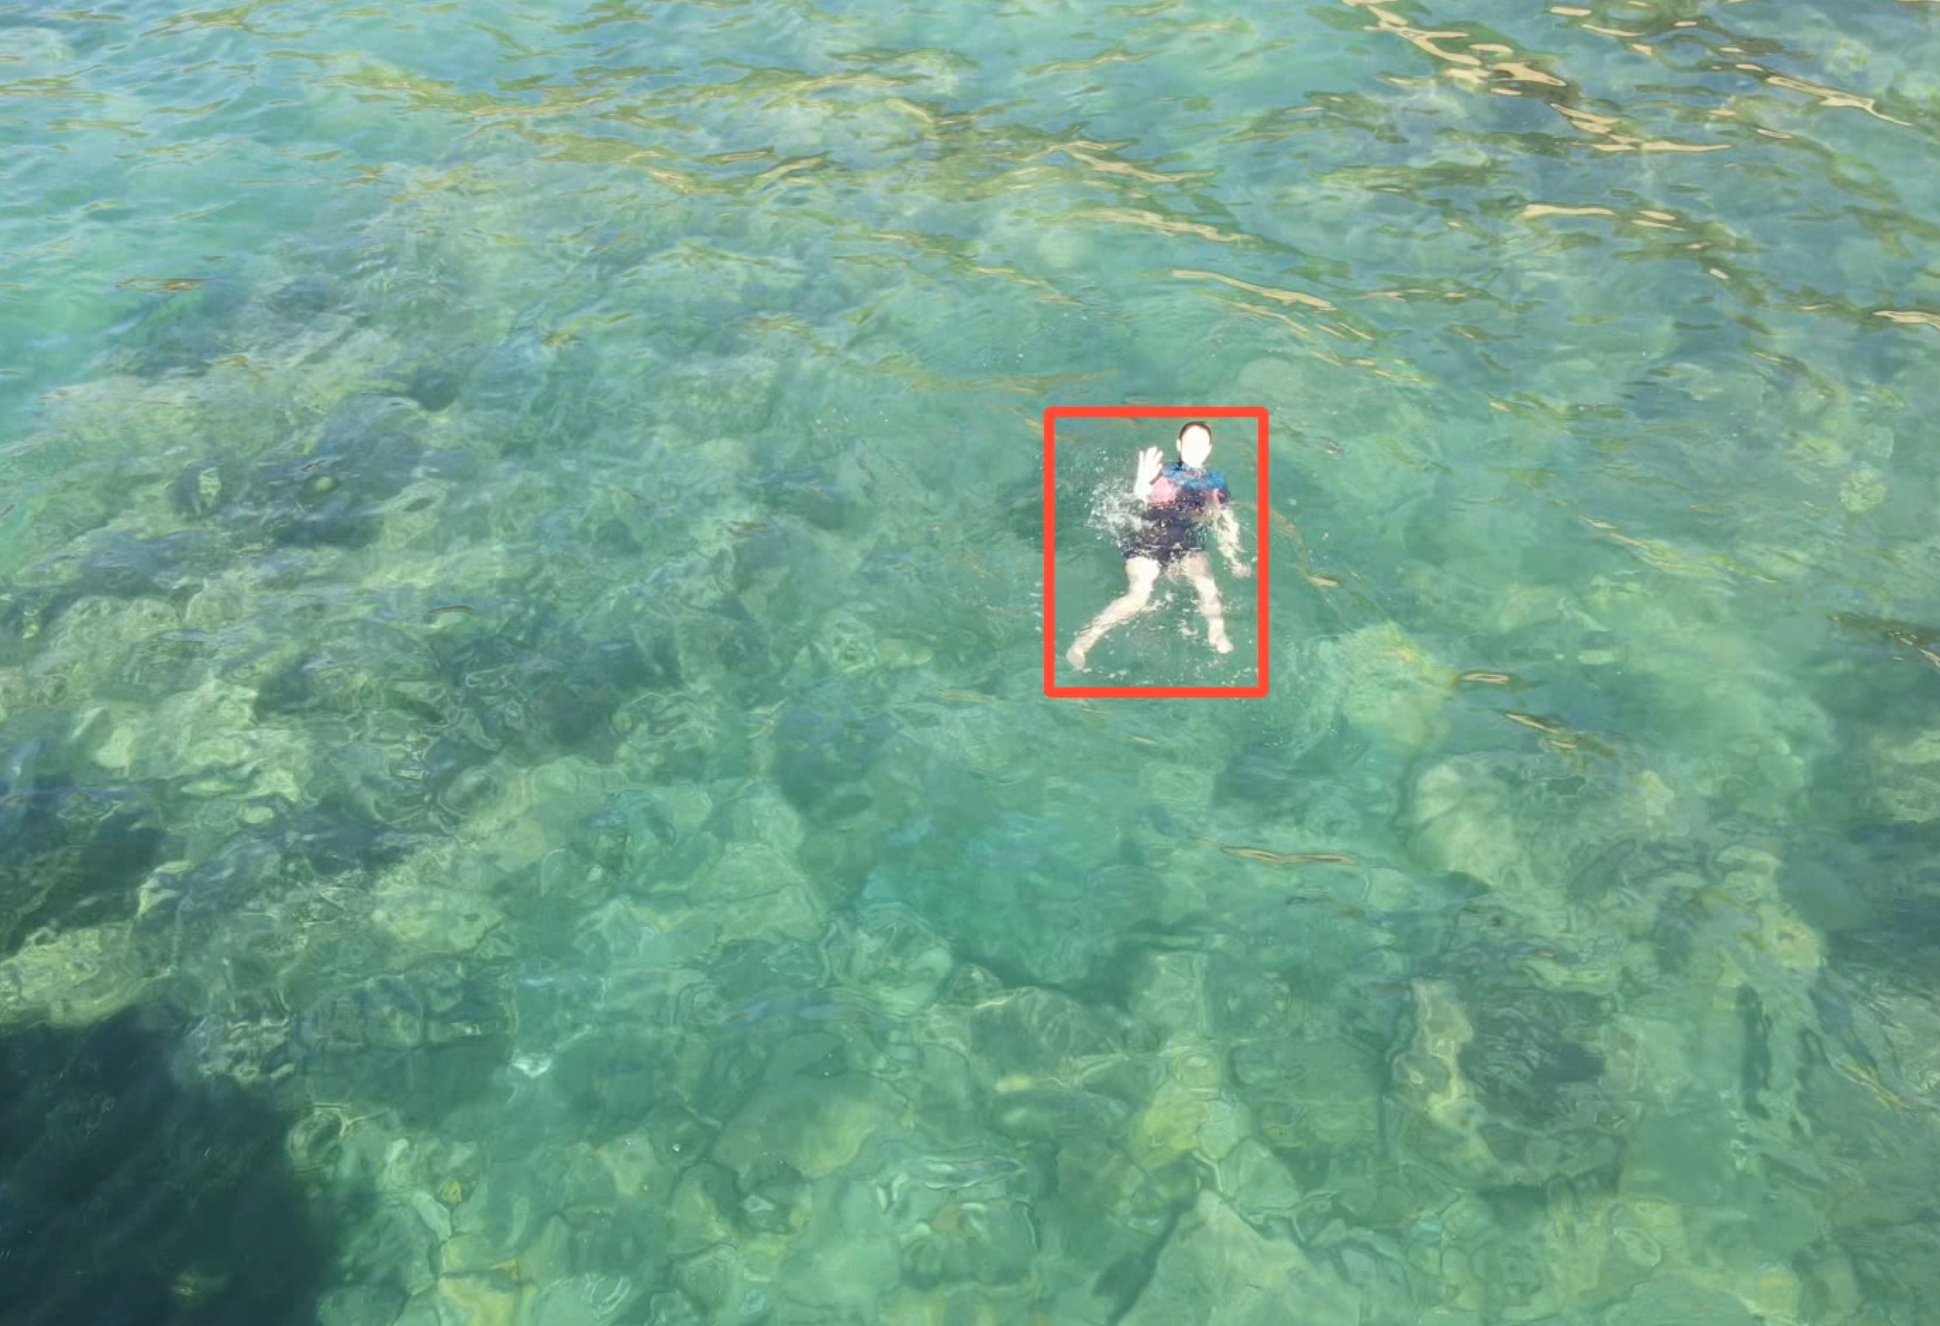
\includegraphics[height=4cm]{figures/det.png}
        \caption{Image après détection du noyé}
        \label{detect}
    \end{minipage}
\end{figure}

Nous avons choisi la version "medium" de YOLOv8, car elle offre un bon compromis entre le nombre de paramètres et la performance de détection. Ensuite, nous avons fait tourner l'algorithme sur quelques vidéos inconnues du modèle sur une GTX 1070 et ainsi pu détecter les zones où se trouvaient des personnes dans l'eau, ainsi qu'un pourcentage de confiance.\newline

Les résultats étaient excellents grâce aux conditions de visibilité quasi identiques à l'apprentissage, mais nous pouvons sans problème étendre la base de données en changeant d'endroit, d'heure et de météo afin de garantir une détection optimale pour toutes les conditions. Nous sommes conscients que nous n'aurons pas une puissance de calcul aussi importante qu'une GTX 1070 sur notre drone en raison des coûts et du poids. Cependant, il reste des étapes importantes d'optimisation telles que la quantification et l'élagage, le passage de python à OpenCV en C++. De plus, nous ne sommes pas contraints de faire tourner le modèle à 60 fps, car les images seront sensiblement les mêmes. En cas de temps de traitement trop long, nous pouvons toujours passer à un modèle plus léger, mais dans notre cas, il est préférable de prendre plus de temps pour faire une inférence plutôt que mettre peu de temps, et avoir des détections manquées.\newline

Une vidéo présente les résultats obtenus sur le lien suivant :
\textcolor{red}{mettre lien yt}

\section{Système de largage}
\label{larg}
Le système de largage doit remplir deux objectifs :

\begin{itemize}
    \item Maintenir la charge utile durant le vol et les manœuvres.
    \item Larguer la charge utile de manière sûre.
    \item Pouvoir tracter la charge utile jusqu’au nageur si elle se déporte lors de son largage.\newline
\end{itemize}

Avant de répondre à ces critères, nous avons dû décider où positionner la charge. Nous avons choisi de la placer sous le fuselage plutôt qu’à l’intérieur, cela nous permet en effet de disposer de davantage de volume pour les composants électroniques et d’optimiser le profil de l’appareil. De plus, si l’on veut varier les dimensions de la charge utile, il est plus aisé de fixer cette dernière sous le fuselage, ce qui n'entraînera pas de grosses modifications structurelles. Afin de ne pas affecter de manière importante les déplacements de l’appareil, la charge est disposée au niveau de la clé d’aile, là où nous essayerons de fixer le centre de gravité de l’appareil.\newline

La charge utile dans le cadre de notre mission sera une bouée autogonflante de la marque OneUp. Son étui est un cylindre de 17cm de long pour 5.7cm de diamètre, le tout pour un poids de 370 grammes. Afin de remplir la contrainte de Dassault d’emporter une charge utile de 500 grammes, nous testerons notre largage avec un cylindre de mêmes dimensions que l’étui mais avec une masse de 500 grammes.

\begin{figure}[h]
    \centering
    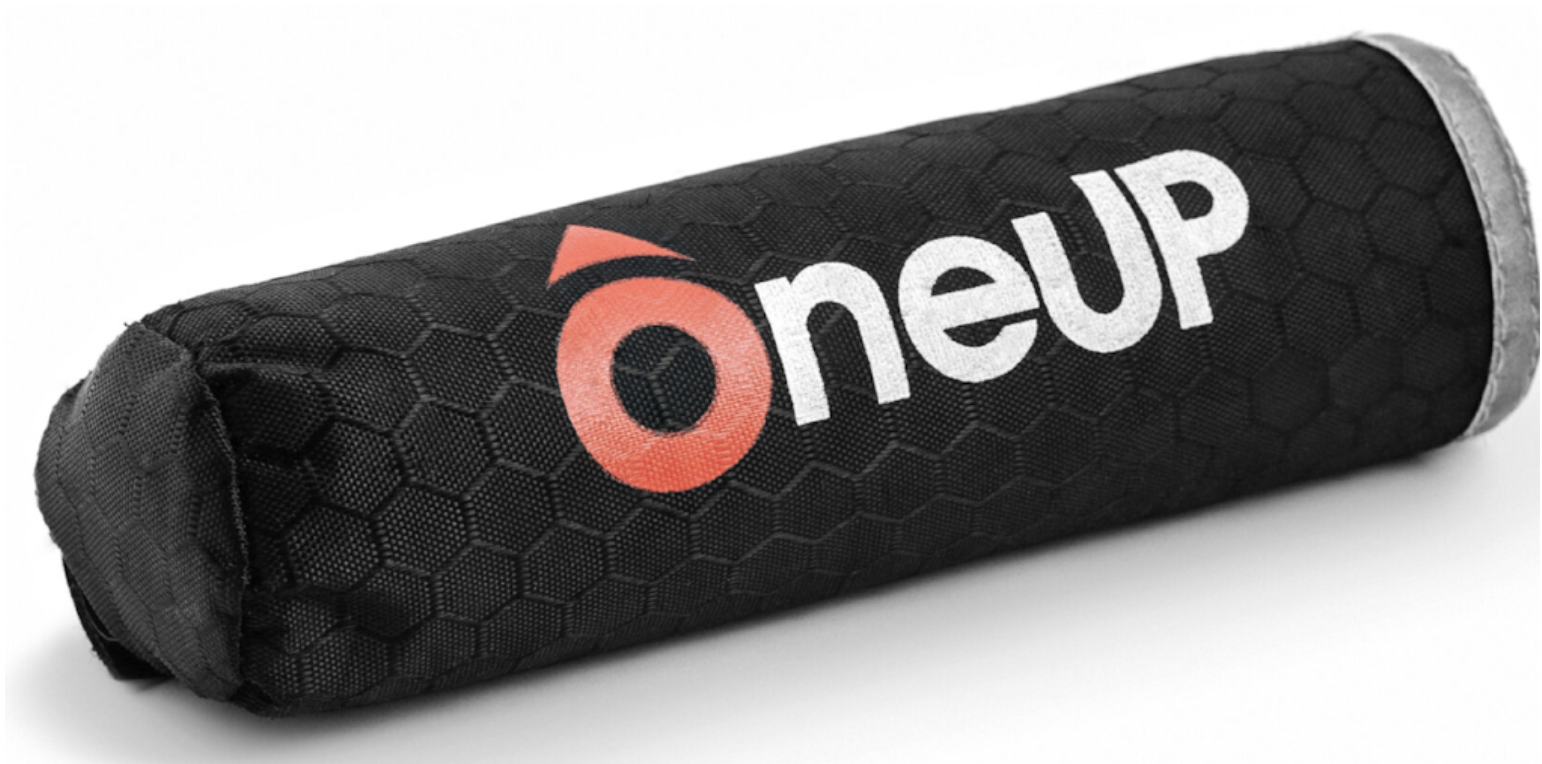
\includegraphics[height=5cm]{figures/bouee.png}
    \caption{title}
\end{figure}

Le système de largage est constitué d’une nacelle placée sous le fuselage. Le système est simple : le servomoteur présent à l’avant de la nacelle manipule un crochet qui, en vol, maintient le plancher de la nacelle fermé. Le plancher sur lequel repose la bouée est donc relié à la nacelle par une liaison pivot libre, et est uniquement retenu en position fermée par la pression exercée par le crochet. Des ressorts le relient également au sommet de la nacelle mais sont insuffisants pour, par leur simple traction, maintenir le plancher fermé lorsque la charge est placée dessus. Dans le cas où lors du largage de la bouée une rafale l’entraînerait loin du nageur en détresse, nous avons fait le choix d’accrocher un fil à la bouée, relié à son autre extrémité par une simple boucle autour du crochet.\newline

\begin{figure}[h]
    \centering
    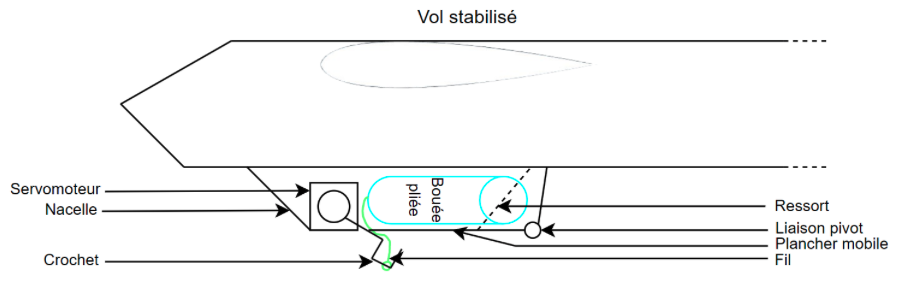
\includegraphics[height=5cm]{figures/b1.png}
    \caption{title}
\end{figure}

Lors du largage, le servomoteur abaisse le crochet afin de libérer la pression contre le plancher, celui-ci s’abaisse alors et la bouée tombe librement. Afin d’éviter que le fil ne se tende lors de la chute et cause des dommages au drone, il faut s’assurer de larguer la charge à une hauteur inférieure à la longueur du fil. La bouée touche alors l’eau et se gonfle seule, toujours maintenue par le fil au crochet.\newline

\begin{figure}[h]
    \centering
    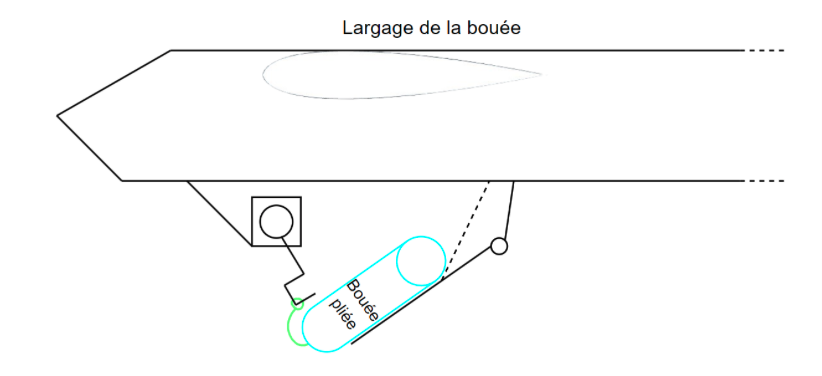
\includegraphics[height=5cm]{figures/b2.png}
    \caption{title}
\end{figure}

Deux cas s’offrent alors : soit la bouée est suffisamment proche du nageur qui la récupère directement, soit la bouée n’a pas atterrit à l’emplacement voulu et il est nécessaire de la tracter vers le nageur (dans la mesure des capacités du drone et de la force des vagues).\newline

\begin{figure}[h]
    \centering
    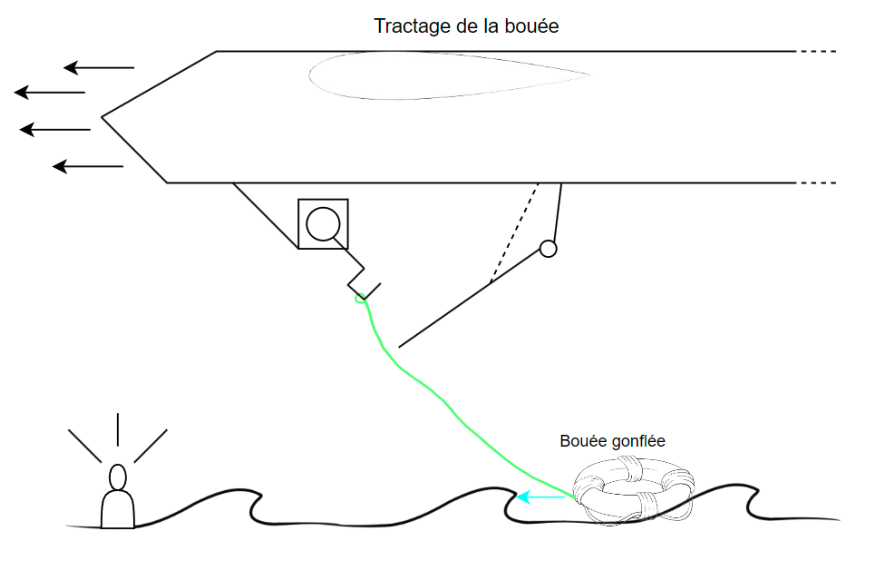
\includegraphics[height=5cm]{figures/b3.png}
    \caption{title}
\end{figure}

Une fois la bouée saisie par le nageur en détresse, le drone abaisse complètement son crochet (sur commande manuelle de l’opérateur) pour libérer le fil et donc la bouée. La présence des ressorts permettent de tirer le plancher de la nacelle vers le haut. Il est ensuite verrouillé par le crochet qui retourne dans sa position initiale. Le drone peut alors revenir sans risques à son point de départ.\newline

\begin{figure}[h]
    \centering
    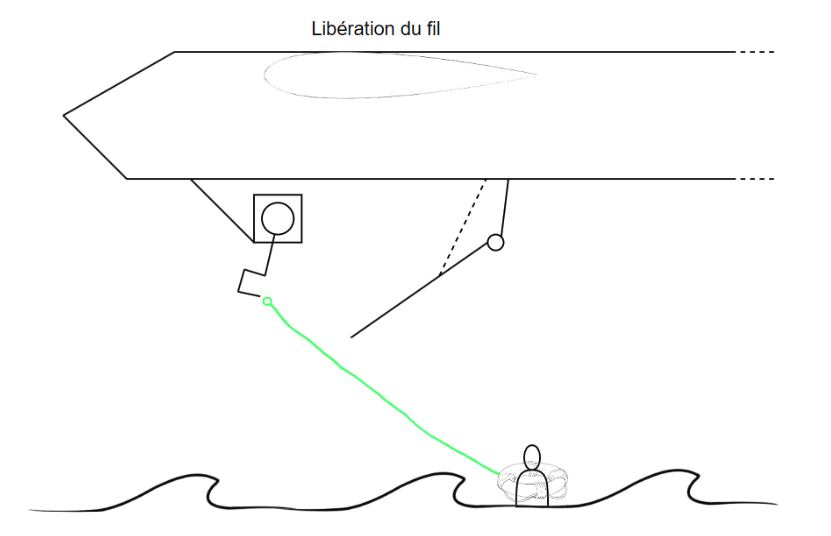
\includegraphics[height=5cm]{figures/b4.png}
    \caption{title}
\end{figure}

Cette nacelle sera placée de manière à ce que son centre de masse (lorsqu’elle est chargée) soit sur le même axe vertical que le centre de gravité de l’appareil, soit au niveau de la clé d’aile. Le tout afin d’influencer le moins possible le comportement en vol horizontal stabilisé du drone. Il faudra dès lors prendre en compte qu’une fois la bouée larguée, le centre de masse de la nacelle se déplacera légèrement vers l’avant (dû au poids du servomoteur) et provoquera un léger moment à piquer, ce qui est préférable à un moment à cabrer.

\chapter{Estimation du coût}

\chapter{État d'avancement du prototype}

\chapter*{Conclusion}
\addcontentsline{toc}{chapter}{\protect\numberline{}Conclusion}


\end{document}